\documentclass[tikz,border=10pt]{standalone}
\usetikzlibrary{arrows.meta, positioning, calc, decorations.pathreplacing}
\usepackage{amsmath}
\usepackage{amssymb}

\begin{document}
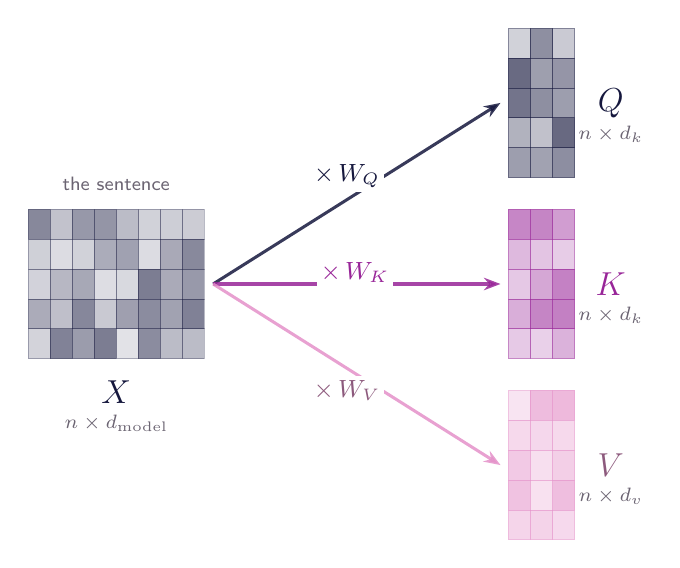
\begin{tikzpicture}[
    every node/.style={font=\sffamily},
]

\definecolor{c1}{HTML}{15173D}   % the sentence, and the queries
\definecolor{c2}{HTML}{982598}   % the keys
\definecolor{c3}{HTML}{E491C9}   % the values
\definecolor{c4}{HTML}{F1E9E9}
\definecolor{axiscolor}{HTML}{333333}
\definecolor{labelcolor}{HTML}{6B6472}

\def\cw{0.28}
\def\ch{0.38}

% ================================================================
%   X   top-left (0, 3.3),   5 rows x 8 cols   (d_model = 8)
%   Q   top-left (6.1, 5.6), 5 rows x 3 cols   (d_k = 3)
%   K   top-left (6.1, 3.3)
%   V   top-left (6.1, 1.0)
% ================================================================

% ---------------------------------------------------------------- X
\foreach \r in {0,...,4} {
    \foreach \c in {0,...,7} {
        \pgfmathsetmacro{\op}{0.12 + 0.45*rnd}
        \fill[c1, opacity=\op] (\c*\cw, 3.3-\r*\ch-\ch) rectangle ++(\cw, \ch);
        \draw[c1, opacity=0.3, line width=0.3pt]
            (\c*\cw, 3.3-\r*\ch-\ch) rectangle ++(\cw, \ch);
    }
}
\node[font=\sffamily\large, text=c1] at (1.12, 0.98) {$X$};
\node[font=\sffamily\scriptsize, text=labelcolor] at (1.12, 0.58)
    {$n \times d_{\mathrm{model}}$};
\node[font=\sffamily\scriptsize, text=labelcolor] at (1.12, 3.62)
    {the sentence};

% ---------------------------------------------------------------- Q, K, V
% fill colour and label colour are separate: c3 is right for the cells but
% too light for text at this size
\foreach \name/\col/\tcol/\ytop/\lbl in {%
    Q/c1/c1/5.6/{$n \times d_k$},
    K/c2/c2/3.3/{$n \times d_k$},
    V/c3/{c3!62!black}/1.0/{$n \times d_v$}} {
  \foreach \r in {0,...,4} {
    \foreach \c in {0,1,2} {
      \pgfmathsetmacro{\op}{0.15 + 0.5*rnd}
      \fill[\col, opacity=\op] (6.1+\c*\cw, \ytop-\r*\ch-\ch) rectangle ++(\cw, \ch);
      \draw[\col, opacity=0.4, line width=0.3pt]
          (6.1+\c*\cw, \ytop-\r*\ch-\ch) rectangle ++(\cw, \ch);
    }
  }
  \node[font=\sffamily\large, text=\tcol] at (7.4, \ytop-0.95)
      {$\name$};
  \node[font=\sffamily\scriptsize, text=labelcolor] at (7.4, \ytop-1.35) {\lbl};
}

% ---------------------------------------------------------------- projections
\foreach \ytarget/\col/\wname/\wshape in {%
    4.65/c1/{W_Q}/{$d_{\mathrm{model}} \times d_k$},
    2.35/c2/{W_K}/{$d_{\mathrm{model}} \times d_k$},
    0.05/c3/{W_V}/{$d_{\mathrm{model}} \times d_v$}} {
  \draw[-{Stealth[length=6pt]}, line width=1.1pt, \col, opacity=0.85]
      (2.35, 2.35) -- (6.0, \ytarget);
}

\node[font=\sffamily\small, text=c1, fill=white, inner sep=1.5pt]
    at (4.05, 3.72) {$\times\, W_Q$};
\node[font=\sffamily\small, text=c2, fill=white, inner sep=1.5pt]
    at (4.15, 2.5) {$\times\, W_K$};
\node[font=\sffamily\small, text=c3!62!black, fill=white, inner sep=1.5pt]
    at (4.05, 1.0) {$\times\, W_V$};

\end{tikzpicture}
\end{document}
